% =====================================================================
% Problema: «montaña rusa eléctrica». Versión del problema 3 del examen
% del capítulo 3 (item:montana) con una esfera cargada que se mueve por
% una vía dentro de un campo eléctrico uniforme.
%
% Formato del examen (restrepo/fundamentacion_en_fisica_parcial_2_2025-2):
% va dentro del \begin{enumerate} de los ítems y usa el entorno solution.
% Requiere: amsmath, siunitx (v3), cancel y tikz (ya cargados allí).
% =====================================================================

\item\label{item:montana-electrica} Una esfera pequeña de masa $m=\qty{2.0}{\g}$ y carga $q=+\qty{2.0}{\micro\coulomb}$ se mueve sin fricción por una vía que está sobre una mesa horizontal, dentro de una región donde hay un campo eléctrico uniforme de magnitud $E=\qty{5.0e3}{\N/\coulomb}$. La figura muestra la vía vista desde arriba: el campo apunta hacia abajo en la figura y las distancias se miden, en contra del campo, desde la recta que pasa por $B$. La esfera parte del reposo en $A$. Como la mesa es horizontal, el peso no influye en el movimiento.

\begin{center}
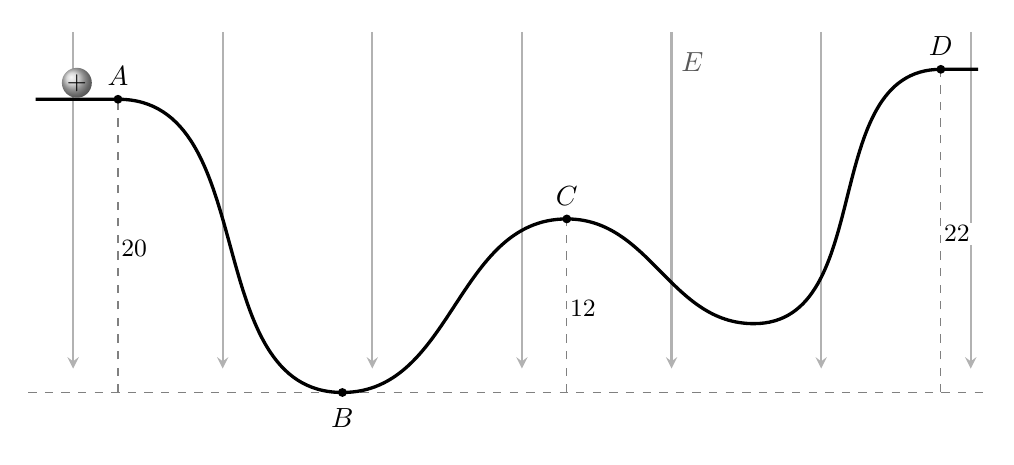
\begin{tikzpicture}[x=0.95cm,y=0.95cm,>=stealth]
    % campo eléctrico uniforme
    \foreach \x in {-0.6,1.4,...,11.4} {
        \draw[->, gray!60, thick] (\x,4.9) -- (\x,0.4);
    }
    \node[gray!70!black, right] at (7.4,4.5) {$\boldsymbol{E}$};
    % recta de referencia por B
    \draw[dashed, gray] (-1.2,0.08) -- (11.6,0.08);
    % vía
    \draw[very thick] (-1.1,4) -- (0,4) to[out=0,in=180] (3,0.08) to[out=0,in=180] (6,2.4)
        to[out=0,in=180] (8.5,1) to[out=0,in=180] (11,4.4) -- (11.5,4.4);
    % distancias medidas en contra del campo
    \foreach \x/\y/\p/\h in {0/4/A/{20}, 6/2.4/C/{12}, 11/4.4/D/{22}} {
        \draw[dashed, gray] (\x,0.08) -- (\x,\y);
        \fill (\x,\y) circle (1.6pt);
        \node[above] at (\x,\y+0.05) {$\p$};
        \node[right, font=\small, fill=white, inner sep=1pt] at (\x,\y/2) {$\qty{\h}{\cm}$};
    }
    \fill (3,0.08) circle (1.6pt);
    \node[below] at (3,0.0) {$B$};
    % esfera en A
    \shade[ball color=gray!40] (-0.55,4.22) circle (0.2);
    \node[font=\small] at (-0.55,4.22) {$+$};
\end{tikzpicture}
\end{center}

\begin{enumerate}
    \item Calcule la rapidez de la esfera en $B$ y en $C$.
    \item ¿Llega la esfera hasta $D$, a $\qty{22}{\cm}$? ¿Hasta qué distancia de la recta de $B$ puede llegar?
    \item ¿Cambian las respuestas anteriores si la esfera tiene el doble de masa y la misma carga? Compare con la montaña rusa del problema~\ref{item:montana}, donde la masa se cancela.
\end{enumerate}

\begin{solution}
La fuerza eléctrica, $q\boldsymbol{E}$, es constante, como el peso cerca de la Tierra. Su energía potencial es $U = qEy$, donde $y$ es la distancia medida en contra del campo (el papel de la altura). Sin fricción, y como la normal no hace trabajo, se conserva la energía mecánica:
\begin{align}
    \frac{1}{2}mv^2 + qEy =& qEy_A\,, \nonumber\\
    v =& \sqrt{\frac{2qE}{m}\,(y_A - y)}\,.
\end{align}
El factor $qE/m$ es la aceleración que produce el campo:
\begin{align}
    \frac{qE}{m} = \frac{(\qty{2.0e-6}{\coulomb})(\qty{5.0e3}{\N/\coulomb})}{\qty{2.0e-3}{\kg}} = \qty{5.0}{\m/\s^2}\,.
\end{align}
\begin{enumerate}
    \item $v_B=\sqrt{2(5.0)(0.20)}\,\unit{\m/\s}\approx\qty{1.41}{\m/\s}$ y $v_C=\sqrt{2(5.0)(0.20-0.12)}\,\unit{\m/\s}\approx\qty{0.89}{\m/\s}$. Comprobación con la energía: el campo hace un trabajo $W = qE\,(\qty{0.20}{\m}) = \qty{2.0e-3}{\joule}$ de $A$ a $B$, y $\tfrac{1}{2}(\qty{2.0e-3}{\kg})(\qty{1.41}{\m/\s})^2 \approx \qty{2.0e-3}{\joule}$.
    \item No: para llegar a $D$ necesitaría una energía potencial $qE\,(\qty{22}{\cm})$, mayor que toda la que tiene, $qE\,(\qty{20}{\cm})$. Llega hasta $\qty{20}{\cm}$, se detiene y regresa. Esta conclusión no depende de $q$, $m$ ni $E$: solo de la distancia de partida.
    \item Las distancias que alcanza no cambian, porque en (b) solo se comparan energías potenciales. Las rapideces sí cambian: $qE/m$ se reduce a la mitad y $v\propto 1/\sqrt{m}$, así que $v_B\approx\qty{1.00}{\m/\s}$ y $v_C\approx\qty{0.63}{\m/\s}$. En la montaña rusa la masa se cancela porque el peso, $mg$, es proporcional a la masa; la fuerza eléctrica, $qE$, depende de la carga y no de la masa. Por eso, en un campo eléctrico, objetos con la misma carga y distinta masa no se mueven igual.
\end{enumerate}
\end{solution}
